\subsection{Dimensionnement du vecteur de vol}
\label{subsec:dimentionnement}

\subsubsection{Méthodologie}
\label{subsubsec:dimentionnement_methode}

Le dimensionnement de la fusée SP-02 a été réalisée en utilisant deux outils principaux : \gls{Stabtraj} et \gls{OpenRocket}. Ces
logiciels permettent de modéliser la fusée, d'analyser ses caractéristiques aérodynamiques et de simuler son comportement en vol.
La méthodologie suivie comprend les étapes suivantes:

\vspace{0.3cm}

\hspace*{-\parindent}%
\begin{minipage}{0.75\textwidth}
    \begin{enumerate}
        \item \textbf{Modélisation \acrshort{CAO} :} La fusée SP-02 a été modélisée en détail dans un logiciel de \acrshort{CAO},
        en tenant compte des dimensions, de la géométrie et de la répartition des masses de chaque composant.
        
        \item \textbf{Importation dans \gls{OpenRocket} :} Après avoir finalisé la modélisation \acrshort{CAO}, le modèle a été
        construit dans le logiciel \gls{OpenRocket} à partir de ces briques de construction. Cette étape permet essentiellement de
        placer les différents éléments de la fusée et de leur attribuer des matériaux. Cela permet de définir la masse et le
        \acrfull{CdG} de chaque élément et donc de la fusée dans son ensemble. Aussi, \gls{OpenRocket} permet d'estimer les
        caractéristiques aérodynamiques de la fusée, telles que le coefficient de traînée ($C_d$), le coefficient de portance
        ($C_l$) et le \acrfull{CdP}, en fonction de la géométrie et des conditions de vol.

        \item \textbf{Importation dans le \gls{Stabtraj} :} Le modèle de la fusée a ensuite été importé dans le \gls{Stabtraj} en
        comptant la masse et le \acrshort{CdG} ainsi que le $C_d$ fournis par \gls{OpenRocket}. En utilisant ces données, le
        \gls{Stabtraj} permet de calculer le \acrshort{CdP} à partir de l'approximation de Barrowman \cite{Stab_doc} et d'analyser
        la stabilité longitudinale de la fusée.

        \item \textbf{Correction et itérations :} Si les résultats de l'analyse de stabilité indiquent que la fusée n'est pas
        stable, des ajustements sont effectués sur la conception, tels que le déplacement du \acrshort{CdG} ou la modification de
        la géométrie des surfaces de portances. La nouvelle conception est ensuite réévaluée en répétant les étapes précédentes
        jusqu'à obtenir une stabilité satisfaisante.
    \end{enumerate}

    \vspace{-0.5cm}

    \subsubsection{Configuration générale adoptée}
    Après plusieurs itérations de conception et d'analyses, nous avons abouti à une configuration générale composée d'un jeu de 4
    ailerons de type trapezoïdal sur chaque étage, une coiffe conique, un changement de diamètre entre les deux étages et un
    rétreint au niveau du bas du premier étage.\\

    Bien que le nombre d'ailerons soit le même pour les deux étages, entrainant le questionnement de l'effet de masquage des
    surfaces portantes du premier étage par le second, le choix a été fait de non pas aligner ces deux jeux d'ailerons mais de les
    décaler de 15° l'un par rapport à l'autre. Ceci répond directemnt à la règle STAB6 du \acrshort{CDC} et à sa partie "contrôle" :

    \begin{quote}
        (Règle) \textit{"STAB6 : Dans le cas d’une fusée à deux jeux d’ailerons dont les ailerons sont alignés, la fusée doit être
        stable à la fois sans tenir compte des effets de masquage du jeu d’aileron inférieur par le jeu d’aileron supérieur et à la
        fois en tenant compte de cette interaction.}\newline\cite[p.~34]{CDC_BiEtage}
    \end{quote}

    \begin{quote}
        (Contrôle) \textit{"STAB6 : On considère que deux jeux d’ailerons sont alignés s’il est possible, vue du vent relatif, de
        trouver deux ailerons consécutifs séparés par un angle de 10° ou moins.}\newline\cite[p.~34]{CDC_BiEtage}
    \end{quote}

    Le choix de ces 15° de décalage permet donc de s'affranchir de cette règle et de simplifier les analyses de stabilité. Cela
    entraine néanmoins une légère diminution de la place disponible entre les ailerons de la fusée et la rampe de lancement car nous
    passons d'un angle de 90° entre deux ailerons consécutifs à un angle de 75°. Cette diminution a été jugée acceptable au regard
    des bénéfices apportés par ce décalage.
\end{minipage}
\hfill
\begin{minipage}{0.20\textwidth}
    \begin{figure}[H]
        \centering
        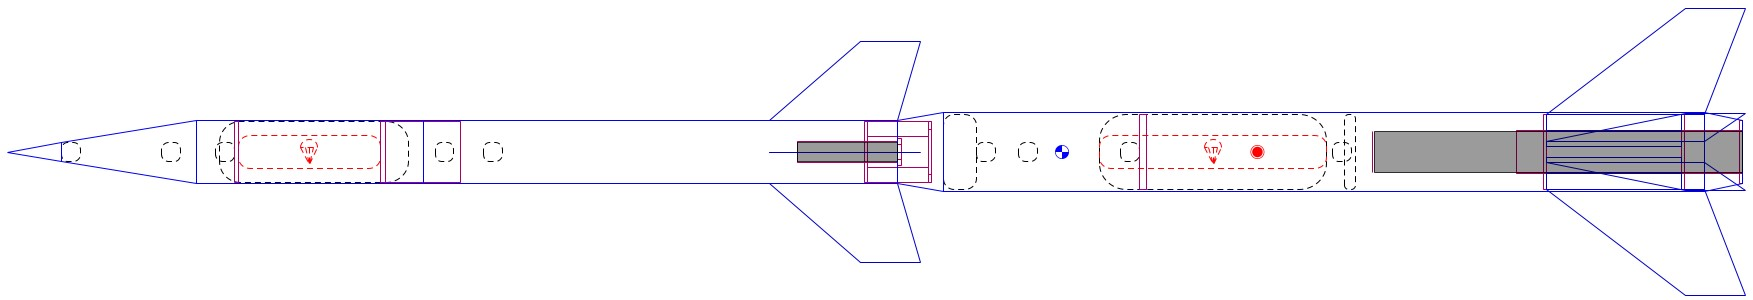
\includegraphics[angle=-90, width=\textwidth]{figures/sp02_ork_f85.jpg}
        \caption{Modélisation de la fusée SP-02 dans \gls{OpenRocket}}
        \label{fig:sp02_ork_model_24-3G}
    \end{figure}
\end{minipage}

\newpage

\subsubsection{Configurations étudiées}
\label{subsubsec:dimentionnement_configurations}

\hspace*{-\parindent}%
\begin{minipage}{0.5\textwidth}
    SP-02 a été conçue selon les règles et le Stabtraj pour une participation au \gls{C'Space} mais également dans l'optique
    d'effectuer des vols plus ambitieux par la suite via d'autre campagnes de lancement. Pour cela, nous avons étudié plusieurs
    configurations de moteurs afin d'optimiser les performances de la fusée et d'assurer sa stabilité dans différentes conditions
    de vol. Dans nos choix, nous nous sommes focalisés sur les configurations présenté dans le tableau
    \ref{tab:configurations_moteurs}.
\end{minipage}
\hfill
\begin{minipage}{0.45\textwidth}
    \begin{table}[H]
        \centering
        \begin{tabular}{l|l|l}
            \hline
            \textbf{Conf.} & \textbf{Moteur Etage 1} & \textbf{Moteur Etage 2} \\
            \hline
            1 & \verb|Pro54-5G-K570|    & \verb|Pro24-3G-F85|*  \\
            2 & \verb|Pro54-5G-K570|    & \verb|Pro38-5G-J285|  \\
            3 & \verb|Pro54-5G-K570|    & \verb|Pro54-5G-K570|  \\
            4 & \verb|Pro54-5G-K1200|   & \verb|Pro54-5G-K1200| \\
            \hline
        \end{tabular}
        \caption{Liste des configurations moteurs étudiés}
        \label{tab:configurations_moteurs}
    \end{table}
\end{minipage}

(*) A cause des problème d'approvisionnement en moteur de fusée, bien que nous devions à la base voler avec un
\texttt{Pro24-6G-G150}, Planète Sciences nous a demander de changer pour un \texttt{Pro24-3G-F85}.

\vfill

\subsubsection{Détermination du domaine de vol}
\label{subsubsec:domaine_de_vol}

Le dimensionnement aérodynamique garantit la stabilité de la fusée, mais il ne suffit pas à autoriser le vol : encore faut-il
démontrer que la fusée retombera à l'intérieur de l'emprise de la base de lancement, y compris en cas de défaillance. Cette
démonstration constitue le \emph{domaine de vol}.

\vfill

\paragraph*{Cas dimensionnant.} Le scénario retenu est celui de la non-ouverture du parachute : la fusée suit alors une trajectoire
purement balistique et sa portée devient maximale. Ce cas est simulé avec une rampe inclinée à 45°, angle qui maximise la distance
parcourue. Pour chaque configuration moteur, quatre simulations \gls{OpenRocket} sont donc réalisées : le premier et le second
étage, chacun à 80° (angle de tir nominal) et à 45° (cas balistique dégradé). La portée retenue pour la configuration est la plus
grande des quatre, systématiquement obtenue par le second étage à 45°.

\vfill

\paragraph*{Critères d'acceptabilité.} Deux contraintes doivent être satisfaites simultanément. La première porte sur la retombée :
la fusée doit rester dans le périmètre de la base quelle que soit l'issue du vol. La seconde porte sur l'altitude : l'espace
aérien au-dessus de la base est plafonné à 3000~m, plafond que l'apogée nominale (obtenue par le second étage à 80°) ne doit pas
dépasser.\\

\vfill

\hspace*{-\parindent}%
\begin{minipage}{0.4\textwidth}

\paragraph*{Construction du cône de vol.} La portée retenue $R$ définit un disque de rayon $R$ centré sur le pas de tir, à
l'intérieur duquel la fusée est susceptible de retomber quel que soit l'azimut. Ce disque étant en pratique plus grand que la
base, on ne cherche pas à l'y inscrire entièrement mais à restreindre l'azimut de tir : pour chaque direction, on calcule la
distance à laquelle un tir sortirait du périmètre, et on ne retient que les directions pour lesquelles cette distance excède $R$.
Les directions admissibles forment un ou plusieurs secteurs angulaires. Le plus large d'entre eux définit le cône de vol,
caractérisé par son angle d'ouverture et par la surface au sol qu'il couvre (figure~\ref{fig:google_earth_methode}). Une
configuration pour laquelle aucun secteur n'est admissible ne peut pas voler depuis cette base.

\end{minipage}
\hfill
\begin{minipage}{0.58\textwidth}

\begin{figure}[H]
    \centering
    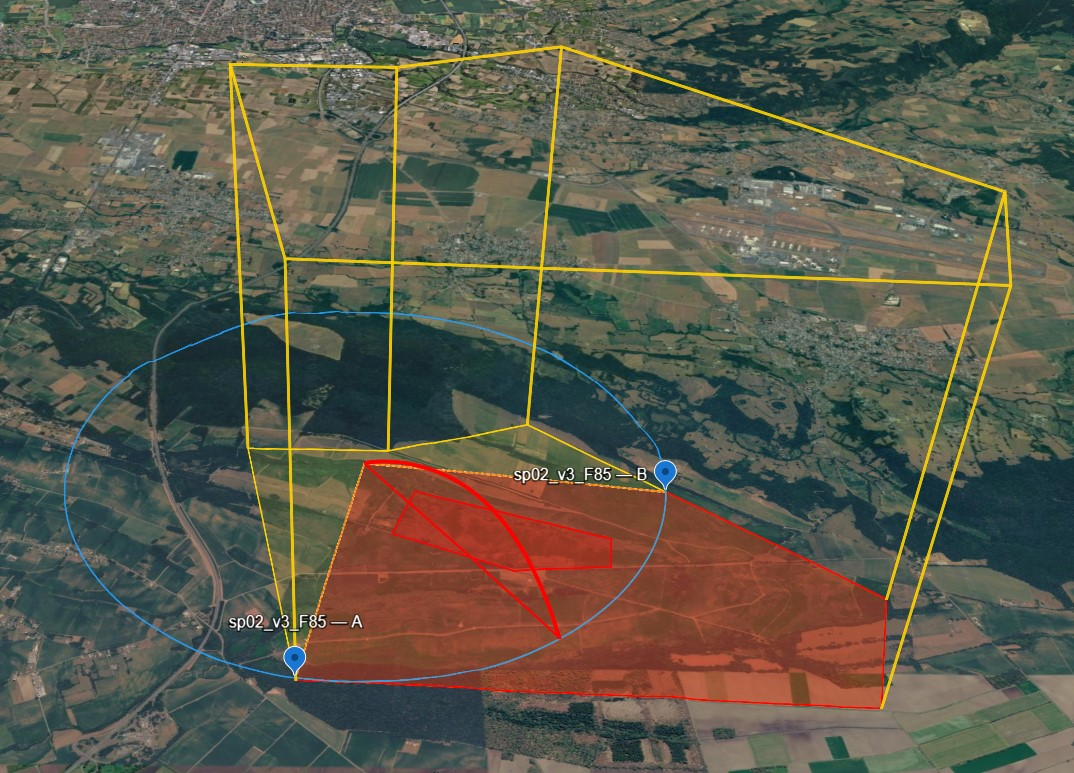
\includegraphics[width=\textwidth]{figures/google_earth/methode.jpg}
    \caption{Détermination du domaine de vol à partir de Google Earth et des données de vol}
    \label{fig:google_earth_methode}
\end{figure}

\end{minipage}

\vfill

\newpage

\subsubsubsection{Configuration 1 : C'Space (Pro54-24)}

\begin{figure}[H]
    \centering
    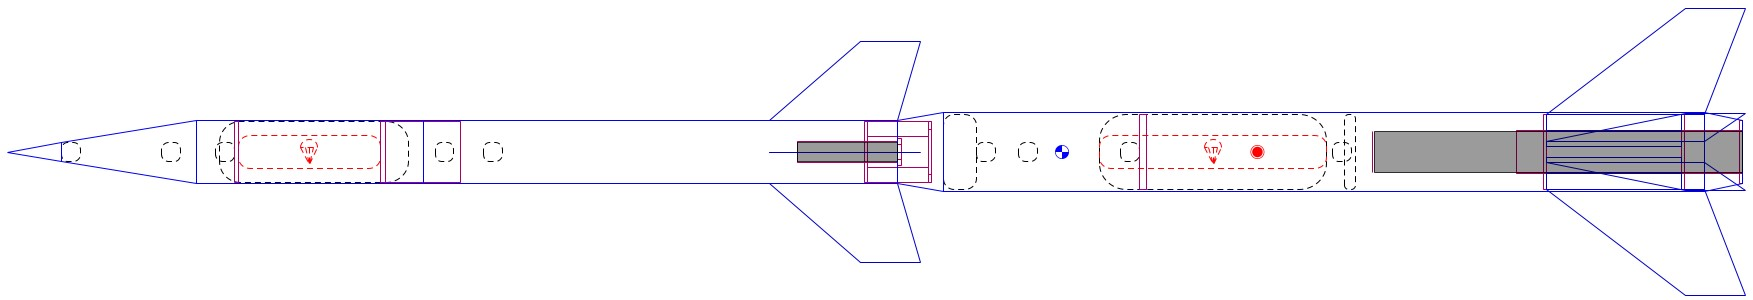
\includegraphics[width=\textwidth]{figures/sp02_ork_f85.jpg}
    \caption{Modélisation dans \gls{OpenRocket} (conf. 1)}
    \label{fig:sp02_ork_model_conf_1}
\end{figure}

Cette configuration est celle effectivement retenue pour le C'Space. Le second étage, propulsé par un \texttt{Pro24-3G-F85},
n'apporte qu'un gain modeste : l'apogée nominale est de 1340~m et la portée balistique de 2143~m. La vitesse maximale atteinte
reste limitée à 171~m/s, soit Mach 0,50 : le vol est intégralement subsonique et la fusée demeure dans le domaine où les
approximations aérodynamiques employées au dimensionnement sont pleinement valides. Cette portée modérée laisse un cône de vol
très ouvert, de 92,9°, couvrant 649,6~ha. L'apogée reste par ailleurs largement sous le plafond de 3000~m.

\begin{figure}[H]
    \centering
    
\includegraphics[width=0.8\textwidth]{figures/sp02_v3_24_3g.png}
    \caption{Vol simulé dans \gls{OpenRocket} (conf. 1)}
    \label{fig:sp02_ork_model_conf_1_vol}
\end{figure}
\begin{figure}[H]
    \centering
    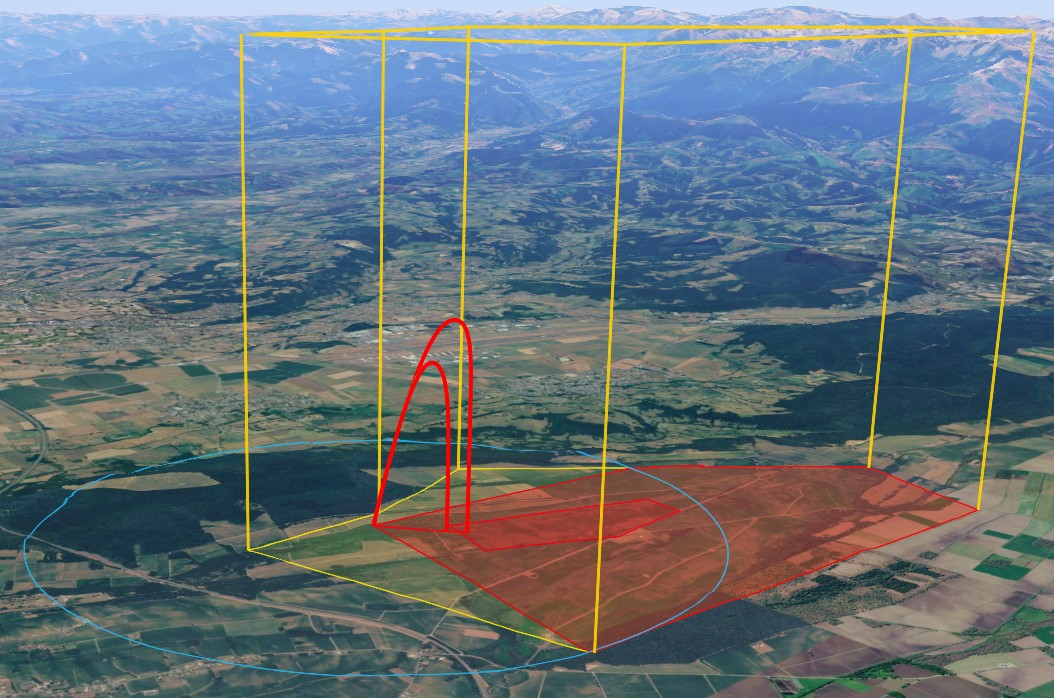
\includegraphics[width=0.8\textwidth]{figures/google_earth/F85.jpg}
    \caption{Domaine de vol dans Google Earth (conf. 1)}
    \label{fig:sp02_google_earth_conf_1}
\end{figure}

% >py analyse_terrain.py etudes/etude_pro24.json -o vues/vue_pro24.json   
% ======================================================================
%   ANALYSE DU DOMAINE DE VOL — Base de lancement de Ger
% ======================================================================

%   Pas de tir
%   ------------------------------------------------------------------
%       rampe_fusex  Rampe FusEx           43.2184361,  -0.0473333   alt   429 m
%       rampe_minif  Rampe Minif           43.2207250,  -0.0522167   alt   433 m

%   Zones
%   ------------------------------------------------------------------
%       perimetre    Périmètre de la base   6 sommets  (décor)   plafond 3000 m
%       zone_rouge   Zone rouge             5 sommets  (décor)

%   Groupes de vols
%   ------------------------------------------------------------------
%       sp02_v3_F85  SP02 F85             4 vol(s)   portée    2143 m   (beta 45 nominal)


%   ==================================================================
%   DOMAINE — SP02 F85
%   ==================================================================
%     Pas de tir      : Rampe FusEx (rampe_fusex)
%     Zone            : Périmètre de la base (perimetre)
%     Portée retenue  : 2143 m   (vol « beta 45 nominal »)
%     Surface de zone : 823.2 ha

%     Distances de sortie de la zone depuis le pas de tir
%     --------------------------------------------------------------
%       azimut   0°   sortie à      820 m   [NON]
%       azimut  30°   sortie à      304 m   [NON]
%       azimut  60°   sortie à      171 m   [NON]
%       azimut  90°   sortie à      146 m   [NON]
%       azimut 120°   sortie à      167 m   [NON]
%       azimut 150°   sortie à      394 m   [NON]
%       azimut 180°   sortie à     1773 m   [NON]
%       azimut 210°   sortie à     3736 m   [OK ]
%       azimut 240°   sortie à     2553 m   [OK ]
%       azimut 270°   sortie à     2149 m   [OK ]
%       azimut 300°   sortie à     1220 m   [NON]
%       azimut 330°   sortie à      850 m   [NON]

%     Secteurs admissibles pour R = 2143 m
%     --------------------------------------------------------------
%        187.9° ->  280.8°   ouverture   92.9°   bissectrice  234.4° <== le plus large

%     RECOMMANDATION
%     --------------------------------------------------------------
%       Azimut de tir   : 234.4°
%       Demi-angle      : ± 46.4°
%       Sortie sur axe  : 2740 m  (marge 596 m)

% ======================================================================
% Vue écrite : vues/vue_pro24.json   (1 domaine(s) sur 1 groupe(s))
%   -> édite-la si besoin, puis : python3 genere_kml.py vues/vue_pro24.json

% >py genere_kml.py vues/vue_pro24.json -o output/pro24.kml
% Zones           : 1   Pas de tir : 1   Domaines : 1
%   [sp02_v3_F85] SP02 F85
%       Pas de tir  : Rampe FusEx (rampe_fusex)   zone Périmètre de la base (perimetre)
%       Cône        : 234.4° ± 46.4°   portée 2143 m   surface 649.6 ha
%       Conformité  : le secteur reste dans la zone
% Trajectoires    :
%   [sp02_v3_F85] SP02 F85   portée groupe 2143 m
%       alpha 80 nominal        150 /  407 pts   apogée    1071 m   portée     463 m   rideau quadrillage_45 (12 segments)
%       beta 80 nominal         150 /  482 pts   apogée    1340 m   portée     590 m   rideau quadrillage_45 (15 segments)
%       alpha 45 nominal        150 /  461 pts   apogée     497 m   portée    1607 m   rideau quadrillage_45 (15 segments)
%       beta 45 nominal         150 /  496 pts   apogée     572 m   portée    2143 m   rideau quadrillage_45 (20 segments)
% KML écrit       : output/pro24.kml

\newpage

\subsubsubsection{Configuration 2 : Pro54-Pro38}
\begin{figure}[H]
    \centering
    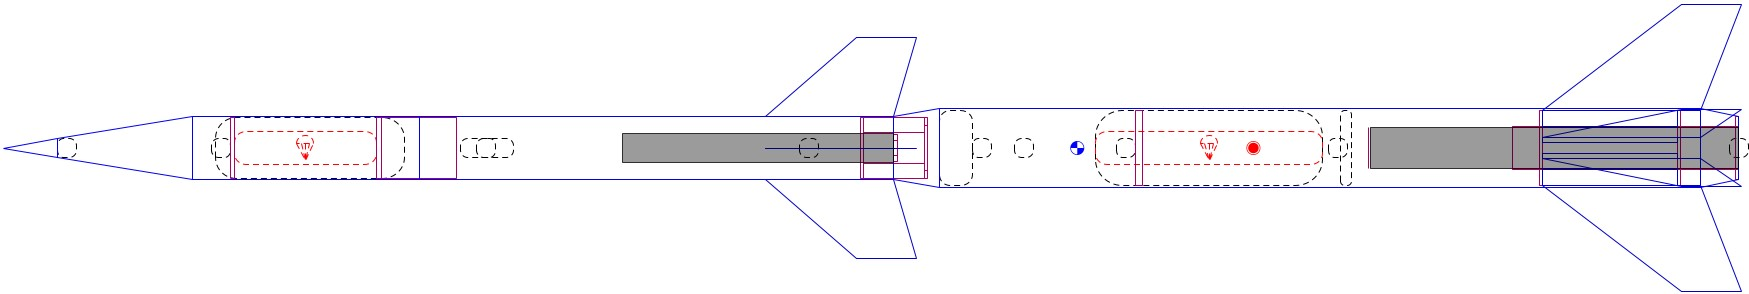
\includegraphics[width=\textwidth]{figures/sp02_ork_j283.jpg}
    \caption{Modélisation dans \gls{OpenRocket} (conf. 2)}
    \label{fig:sp02_ork_model_conf_2}
\end{figure}

Le passage au \texttt{Pro38-5G-J285} fait passer l'apogée nominale à 2191~m et la portée balistique à 3169~m, pour une vitesse
maximale de 246~m/s (Mach 0,72). Le vol reste subsonique, mais s'approche du domaine transsonique. Le domaine reste conforme et se
resserre : le cône a une ouverture de 26,4° pour 301,6~ha.

\begin{figure}[H]
    \centering
    
\includegraphics[width=0.8\textwidth]{figures/sp02_v3_38.png}
    \caption{Vol simulé dans \gls{OpenRocket} (conf. 2)}
    \label{fig:sp02_ork_model_conf_2_vol}
\end{figure}
\begin{figure}[H]
    \centering
    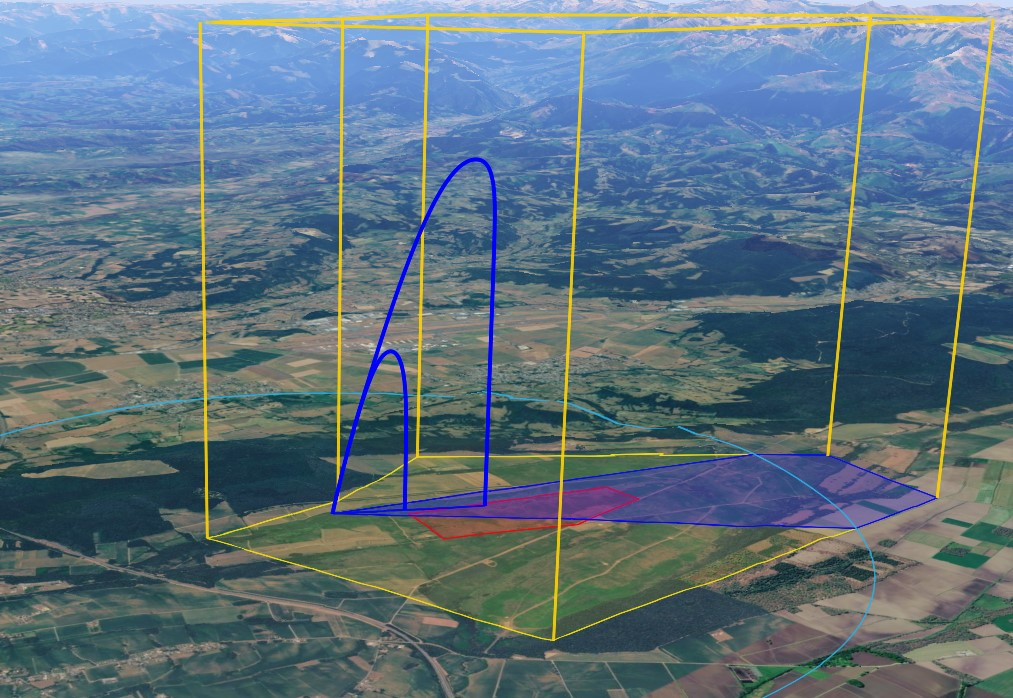
\includegraphics[width=0.8\textwidth]{figures/google_earth/J283.jpg}
    \caption{Domaine de vol dans Google Earth (conf. 2)}
    \label{fig:sp02_google_earth_conf_2}
\end{figure}

% >py analyse_terrain.py etudes/etude_pro38.json -o vues/vue_pro38.json
% ======================================================================
%   ANALYSE DU DOMAINE DE VOL — Base de lancement de Ger
% ======================================================================

%   Pas de tir
%   ------------------------------------------------------------------
%       rampe_fusex  Rampe FusEx           43.2184361,  -0.0473333   alt   429 m
%       rampe_minif  Rampe Minif           43.2207250,  -0.0522167   alt   433 m

%   Zones
%   ------------------------------------------------------------------
%       perimetre    Périmètre de la base   6 sommets  (décor)   plafond 3000 m
%       zone_rouge   Zone rouge             5 sommets  (décor)

%   Groupes de vols
%   ------------------------------------------------------------------
%       sp02_v3_J285 SP02 J285            4 vol(s)   portée    3169 m   (beta 45 nominal)


%   ==================================================================
%   DOMAINE — SP02 J285
%   ==================================================================
%     Pas de tir      : Rampe FusEx (rampe_fusex)
%     Zone            : Périmètre de la base (perimetre)
%     Portée retenue  : 3169 m   (vol « beta 45 nominal »)
%     Surface de zone : 823.2 ha

%     Distances de sortie de la zone depuis le pas de tir
%     --------------------------------------------------------------
%       azimut   0°   sortie à      820 m   [NON]
%       azimut  30°   sortie à      304 m   [NON]
%       azimut  60°   sortie à      171 m   [NON]
%       azimut  90°   sortie à      146 m   [NON]
%       azimut 120°   sortie à      167 m   [NON]
%       azimut 150°   sortie à      394 m   [NON]
%       azimut 180°   sortie à     1773 m   [NON]
%       azimut 210°   sortie à     3736 m   [OK ]
%       azimut 240°   sortie à     2553 m   [NON]
%       azimut 270°   sortie à     2149 m   [NON]
%       azimut 300°   sortie à     1220 m   [NON]
%       azimut 330°   sortie à      850 m   [NON]

%     Secteurs admissibles pour R = 3169 m
%     --------------------------------------------------------------
%        199.0° ->  225.4°   ouverture   26.4°   bissectrice  212.2° <== le plus large

%     RECOMMANDATION
%     --------------------------------------------------------------
%       Azimut de tir   : 212.2°
%       Demi-angle      : ± 13.2°
%       Sortie sur axe  : 3774 m  (marge 605 m)

% ======================================================================
% Vue écrite : vues/vue_pro38.json   (1 domaine(s) sur 1 groupe(s))
%   -> édite-la si besoin, puis : python3 genere_kml.py vues/vue_pro38.json

% >py genere_kml.py vues/vue_pro38.json -o output/pro38.kml
% Zones           : 2   Pas de tir : 2   Domaines : 1
%   [sp02_v3_J285] SP02 J285
%       Pas de tir  : Rampe FusEx (rampe_fusex)   zone Périmètre de la base (perimetre)
%       Cône        : 212.2° ± 13.2°   portée 3169 m   surface 301.6 ha
%       Conformité  : le secteur reste dans la zone
% Trajectoires    :
%   [sp02_v3_J285] SP02 J285   portée groupe 3169 m
%       alpha 80 nominal        150 /  403 pts   apogée    1034 m   portée     459 m   rideau quadrillage_45 (12 segments)
%       beta 80 nominal         150 /  629 pts   apogée    2191 m   portée     975 m   rideau quadrillage_45 (25 segments)
%       alpha 45 nominal        150 /  457 pts   apogée     472 m   portée    1573 m   rideau quadrillage_45 (14 segments)
%       beta 45 nominal         150 /  599 pts   apogée     779 m   portée    3169 m   rideau quadrillage_45 (29 segments)
% KML écrit       : output/pro38.kml

\newpage

\subsubsubsection{Configuration 3 : Pro54-Pro54 (K570)}

\begin{figure}[H]
    \centering
    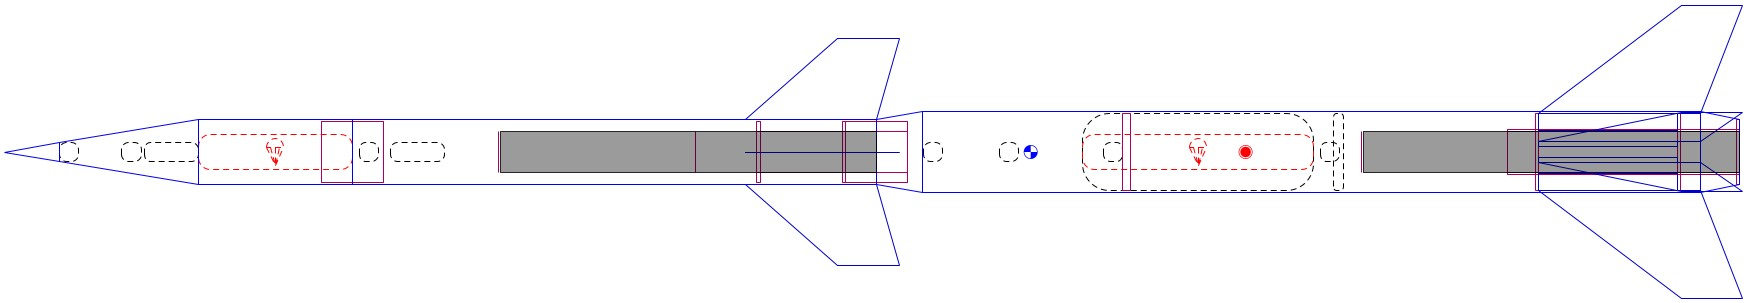
\includegraphics[width=\textwidth]{figures/sp02_ork_k570.jpg}
    \caption{Modélisation dans \gls{OpenRocket}}
    \label{fig:sp02_ork_model_conf_3}
\end{figure}

La configuration symétrique en \texttt{Pro54-5G-K570} porte l'apogée nominale à 3292~m et la portée balistique à 4229~m, avec une
vitesse maximale de 384~m/s. La fusée franchit ici le mur du son (Mach 1,13), ce qui sort du domaine de validité des
approximations retenues au dimensionnement et appellerait une caractérisation aérodynamique dédiée. La configuration est
également non conforme : l'apogée dépasse le plafond de 3000~m (3292~m), et aucun azimut ne permet d'atteindre 4229~m sans sortir
du périmètre. Aucun cône de vol ne peut donc être construit. Cette configuration est écartée pour un tir depuis Ger et
nécessiterait une base offrant une zone de retombée sensiblement plus étendue.

\begin{figure}[H]
    \centering
    
\includegraphics[width=0.7\textwidth]{figures/sp02_v3_54_570.png}
    \caption{Vol simulé dans \gls{OpenRocket}}
    \label{fig:sp02_ork_model_conf_3_vol}
\end{figure}
\begin{figure}[H]
    \centering
    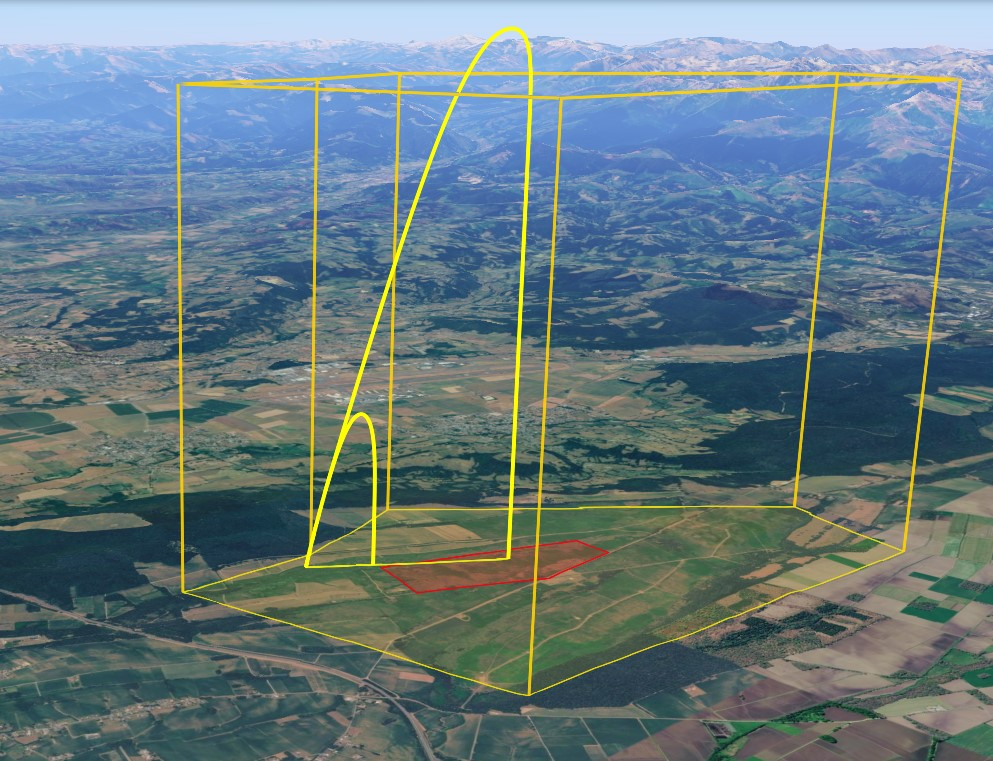
\includegraphics[width=0.7\textwidth]{figures/google_earth/K570.jpg}
    \caption{Domaine de vol dans Google Earth (conf. 3)}
    \label{fig:sp02_google_earth_conf_3}
\end{figure}

% >py analyse_terrain.py etudes/etude_pro54_k570.json -o vues/vue_pro54_k570.json
% ======================================================================
%   ANALYSE DU DOMAINE DE VOL — Base de lancement de Ger
% ======================================================================

%   Pas de tir
%   ------------------------------------------------------------------
%       rampe_fusex  Rampe FusEx           43.2184361,  -0.0473333   alt   429 m
%       rampe_minif  Rampe Minif           43.2207250,  -0.0522167   alt   433 m

%   Zones
%   ------------------------------------------------------------------
%       perimetre    Périmètre de la base   6 sommets  (décor)   plafond 3000 m
%       zone_rouge   Zone rouge             5 sommets  (décor)

%   Groupes de vols
%   ------------------------------------------------------------------
%       sp02_v3_K570 SP02 K570            4 vol(s)   portée    4229 m   (beta 45 nominal)


%   ==================================================================
%   DOMAINE — SP02 K570
%   ==================================================================
%     Pas de tir      : Rampe FusEx (rampe_fusex)
%     Zone            : Périmètre de la base (perimetre)
%     Portée retenue  : 4229 m   (vol « beta 45 nominal »)
%     Surface de zone : 823.2 ha

%     Distances de sortie de la zone depuis le pas de tir
%     --------------------------------------------------------------
%       azimut   0°   sortie à      820 m   [NON]
%       azimut  30°   sortie à      304 m   [NON]
%       azimut  60°   sortie à      171 m   [NON]
%       azimut  90°   sortie à      146 m   [NON]
%       azimut 120°   sortie à      167 m   [NON]
%       azimut 150°   sortie à      394 m   [NON]
%       azimut 180°   sortie à     1773 m   [NON]
%       azimut 210°   sortie à     3736 m   [NON]
%       azimut 240°   sortie à     2553 m   [NON]
%       azimut 270°   sortie à     2149 m   [NON]
%       azimut 300°   sortie à     1220 m   [NON]
%       azimut 330°   sortie à      850 m   [NON]

%     Aucun secteur admissible pour cette portée.

%     [!] aucun azimut ne permet 4229 m sans sortir de la zone (sortie la plus lointaine : 146 m environ) — 'demi_angle_deg' manquant, aucun domaine produit.

% ======================================================================
% [!] groupe « sp02_v3_K570 » : aucun azimut ne permet 4229 m sans sortir de la zone (sortie la plus lointaine : 146 m environ).
%       'azimut_deg' est fixé à 214.6° mais pas 'demi_angle_deg' : impossible de déduire l'ouverture.
%       Aucun domaine produit.
% Vue écrite : vues/vue_pro54_k570.json   (0 domaine(s) sur 1 groupe(s))
%   -> édite-la si besoin, puis : python3 genere_kml.py vues/vue_pro54_k570.json

% >py genere_kml.py vues/vue_pro54_k570.json -o output/pro54_k570.kml
% Zones           : 2   Pas de tir : 2   Domaines : 0   (aucun domaine à dessiner)
% Trajectoires    :
%   [sp02_v3_K570] SP02 K570   portée groupe 4229 m
%       alpha 80 nominal        150 /  394 pts   apogée     993 m   portée     429 m   rideau quadrillage_45 (12 segments)
%       beta 80 nominal         150 /  832 pts   apogée    3292 m   portée    1302 m   rideau quadrillage_45 (38 segments)
%       alpha 45 nominal        150 /  452 pts   apogée     458 m   portée    1492 m   rideau quadrillage_45 (14 segments)
%       beta 45 nominal         150 /  917 pts   apogée    1186 m   portée    4229 m   rideau quadrillage_45 (40 segments)
% [!] aucun domaine dans la vue : seuls les zones, les pas de tir et les trajectoires sont dessinés.
%       Pour en obtenir un, fixe 'azimut_deg' et 'demi_angle_deg' sur le groupe, puis relance l'analyse.
% KML écrit       : output/pro54_k570.kml

\newpage

\subsubsubsection{Configuration 4 : Pro54-Pro54 (K1200)}
blabla
\begin{figure}[H]
    \centering
    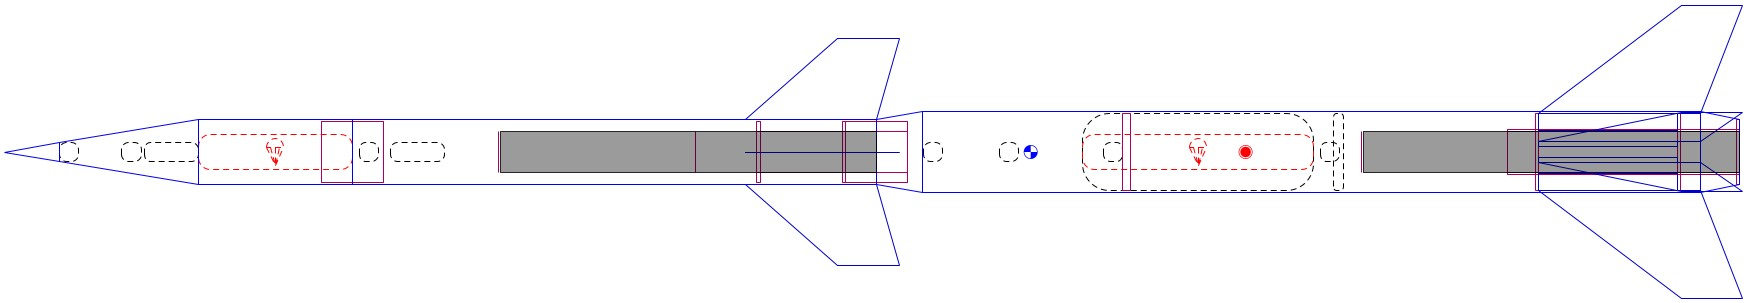
\includegraphics[width=\textwidth]{figures/sp02_ork_k570.jpg}
    \caption{Modélisation dans \gls{OpenRocket}}
    \label{fig:sp02_ork_model_conf_4}
\end{figure}

Le \texttt{Pro54-5G-K1200} délivre une impulsion totale très proche de celle du \texttt{K570}, mais sur une durée bien plus
courte : environ 1,6 à 1,7~s de combustion contre 3,6 à 3,7~s. La vitesse maximale de cette configutation est de 537~m/s, soit
Mach 1,58.

\begin{figure}[H]
    \centering
    
\includegraphics[width=\textwidth]{figures/sp02_v3_54_1200.png}
    \caption{Vol simulé dans \gls{OpenRocket}}
    \label{fig:sp02_ork_model_conf_4_vol}
\end{figure}

Malgré une poussée moyenne plus élevée, cette configuration présente des performances inférieures à celles de la configuration~3 :
l'apogée nominale s'établit à 2990~m et la portée balistique à 3762~m, contre respectivement 3292~m et 4229~m. Ce résultat
s'explique par le régime aérodynamique atteint. À impulsion totale comparable, une combustion deux fois plus courte conduit à des
vitesses sensiblement plus élevées, la traînée croissant avec le carré de la vitesse. S'y ajoute la traînée d'onde, qui apparaît
au franchissement du transsonique et majore le coefficient de traînée dans un rapport de 2 à 3 : la configuration~4 s'établit à
Mach 1,58 tandis que la configuration~3 atteint Mach 1,13. La fraction de l'énergie propulsive dissipée par la traînée est donc
plus importante dans le premier cas.\\

La portée réduite fait réapparaître un secteur admissible, dont l'ouverture est de 6,0° pour une surface de 75,7~ha. L'apogée de
2990~m laisse par ailleurs une marge de 10~m sous le plafond autorisé.

\newpage

\begin{figure}[H]
    \centering
    \includegraphics[width=\textwidth]{figures/google_earth/K1200.jpg}
    \caption{Domaine de vol dans Google Earth (conf. 4)}
    \label{fig:sp02_google_earth_conf_4}
\end{figure}

% >py analyse_terrain.py etudes/etude_pro54_k1200.json -o vues/vue_pro54_k1200.json
% ======================================================================
%   ANALYSE DU DOMAINE DE VOL — Base de lancement de Ger
% ======================================================================

%   Pas de tir
%   ------------------------------------------------------------------
%       rampe_fusex  Rampe FusEx           43.2184361,  -0.0473333   alt   429 m
%       rampe_minif  Rampe Minif           43.2207250,  -0.0522167   alt   433 m

%   Zones
%   ------------------------------------------------------------------
%       perimetre    Périmètre de la base   6 sommets  (décor)   plafond 3000 m
%       zone_rouge   Zone rouge             5 sommets  (décor)

%   Groupes de vols
%   ------------------------------------------------------------------
%       sp02_v3_K1200 SP02 K1200           4 vol(s)   portée    3762 m   (beta 45 nominal)


%   ==================================================================
%   DOMAINE — SP02 K1200
%   ==================================================================
%     Pas de tir      : Rampe FusEx (rampe_fusex)
%     Zone            : Périmètre de la base (perimetre)
%     Portée retenue  : 3762 m   (vol « beta 45 nominal »)
%     Surface de zone : 823.2 ha

%     Distances de sortie de la zone depuis le pas de tir
%     --------------------------------------------------------------
%       azimut   0°   sortie à      820 m   [NON]
%       azimut  30°   sortie à      304 m   [NON]
%       azimut  60°   sortie à      171 m   [NON]
%       azimut  90°   sortie à      146 m   [NON]
%       azimut 120°   sortie à      167 m   [NON]
%       azimut 150°   sortie à      394 m   [NON]
%       azimut 180°   sortie à     1773 m   [NON]
%       azimut 210°   sortie à     3736 m   [NON]
%       azimut 240°   sortie à     2553 m   [NON]
%       azimut 270°   sortie à     2149 m   [NON]
%       azimut 300°   sortie à     1220 m   [NON]
%       azimut 330°   sortie à      850 m   [NON]

%     Secteurs admissibles pour R = 3762 m
%     --------------------------------------------------------------
%        211.6° ->  217.5°   ouverture    6.0°   bissectrice  214.6° <== le plus large

%     RECOMMANDATION
%     --------------------------------------------------------------
%       Azimut de tir   : 214.6°
%       Demi-angle      : ± 3.0°
%       Sortie sur axe  : 3822 m  (marge 59 m)

% ======================================================================
% Vue écrite : vues/vue_pro54_k1200.json   (1 domaine(s) sur 1 groupe(s))
%   -> édite-la si besoin, puis : python3 genere_kml.py vues/vue_pro54_k1200.json

% >py genere_kml.py vues/vue_pro54_k1200.json -o output/pro54_k1200.kml
% Zones           : 2   Pas de tir : 2   Domaines : 1
%   [sp02_v3_K1200] SP02 K1200
%       Pas de tir  : Rampe FusEx (rampe_fusex)   zone Périmètre de la base (perimetre)
%       Cône        : 214.6° ± 3.0°   portée 3762 m   surface 75.7 ha
%       Conformité  : le secteur reste dans la zone
% Trajectoires    :
%   [sp02_v3_K1200] SP02 K1200   portée groupe 3762 m
%       alpha 80 nominal        150 /  354 pts   apogée     878 m   portée     344 m   rideau quadrillage_45 (9 segments)
%       beta 80 nominal         150 /  740 pts   apogée    2990 m   portée     962 m   rideau quadrillage_45 (33 segments)
%       alpha 45 nominal        150 /  435 pts   apogée     470 m   portée    1288 m   rideau quadrillage_45 (12 segments)
%       beta 45 nominal         150 /  823 pts   apogée    1516 m   portée    3762 m   rideau quadrillage_45 (37 segments)
% KML écrit       : output/pro54_k1200.kml

\subsubsubsection{Synthèse}

La configuration 1 est celle retenue pour le C'Space, mais les trois autres configurations ont été étudiées pour évaluer les
performances de la fusée SP-02 et les contraintes de la base de Ger. La synthèse des résultats est présentée dans le tableau
\ref{tab:synthese_domaine_vol}.

\begin{table}[H]
    \centering
    \footnotesize
    \setlength{\tabcolsep}{10pt}
    \begin{tabular}{l|c|c|c|c|c|c}
        \hline
        \textbf{Conf.} & \textbf{$V_{max}$} & \textbf{Apogée} & \textbf{Apogée}
        & \textbf{Portée bal.} & \textbf{Ouverture} & \textbf{Surface} \\
        & & 1\ier{} étage \textbf{(80°)} & 2\ieme{} étage \textbf{(80°)} & \textbf{(45°)} & & \\
        \hline
        1 -- \texttt{F85}   & 171 m/s (M 0,50) & 1071 m & 1340 m & 2143 m & 92,9° & 649,6 ha \\
        2 -- \texttt{J285}  & 246 m/s (M 0,72) & 1034 m & 2191 m & 3169 m & 26,4° & 301,6 ha \\
        3 -- \texttt{K570}  & 384 m/s (M 1,13) &  993 m & 3292 m & 4229 m & \multicolumn{2}{c}{aucun domaine admissible} \\
        4 -- \texttt{K1200} & 537 m/s (M 1,58) &  878 m & 2990 m & 3762 m & 6,0°  & 75,7 ha \\
        \hline
    \end{tabular}
    \caption{Synthèse des domaines de vol sur la base de Ger. Les nombres de Mach sont calculés pour
    l'atmosphère standard au niveau de la mer ($a = 340$~m/s).}
    \label{tab:synthese_domaine_vol}
\end{table}

On constate que bien que les configurations 3 et 4 soient à la limite de la zone de vol autorisée par le camp de Ger voire la
dépassent, la configuration 2 semble être un bon compromis entre performances et contraintes de la base. Un couple
\texttt{Pro54-5G-K570} et \texttt{Pro38-5G-J285} constituerait une configuration de bi-étage performante, légère, de taille
modérée et conforme aux contraintes de la base.

\newpage

\subsubsection{Analyse de stabilité}

De l'étude de stabilité effectué sur la configuration 1, trois graphiques principaux ont été extraits, présentés dans la figure
\ref{fig:stabilite_resultats}. Ces graphiques montrent l'évolution des marges de stabilité longitudinale de la fusée SP-02
complète, du premier étage et du second étage en fonction de la variation de masse de propergol consommée durant le vol.\\

\begin{figure}[h!]
    \centering
    \begin{subfigure}{0.32\textwidth}
        \centering
        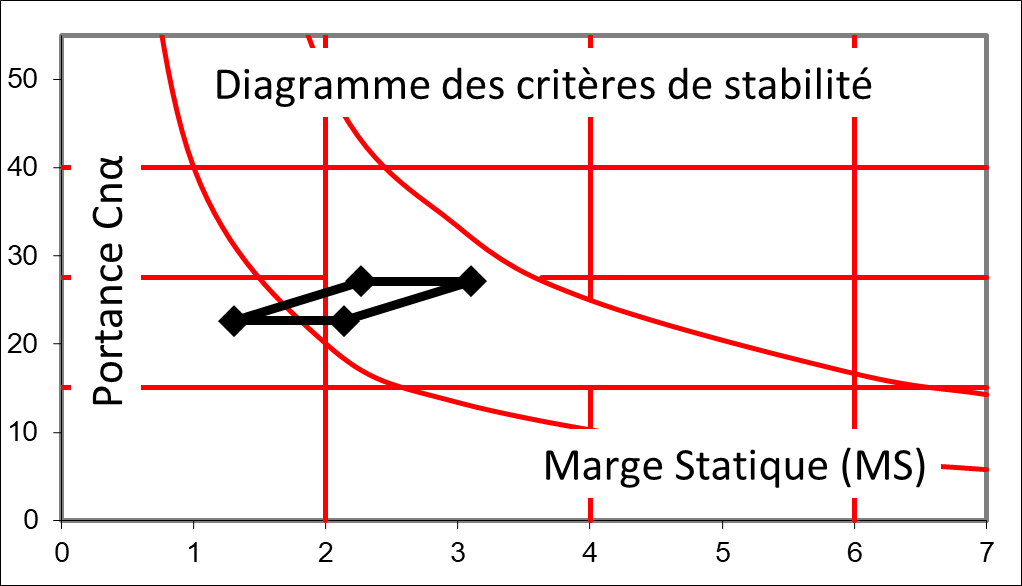
\includegraphics[width=\textwidth]{figures/stabtraj_ensemble.png}
        \caption{Fusée SP-02 complète}
        \label{fig:stabilite_sp02}
    \end{subfigure}
    \begin{subfigure}{0.32\textwidth}
        \centering
        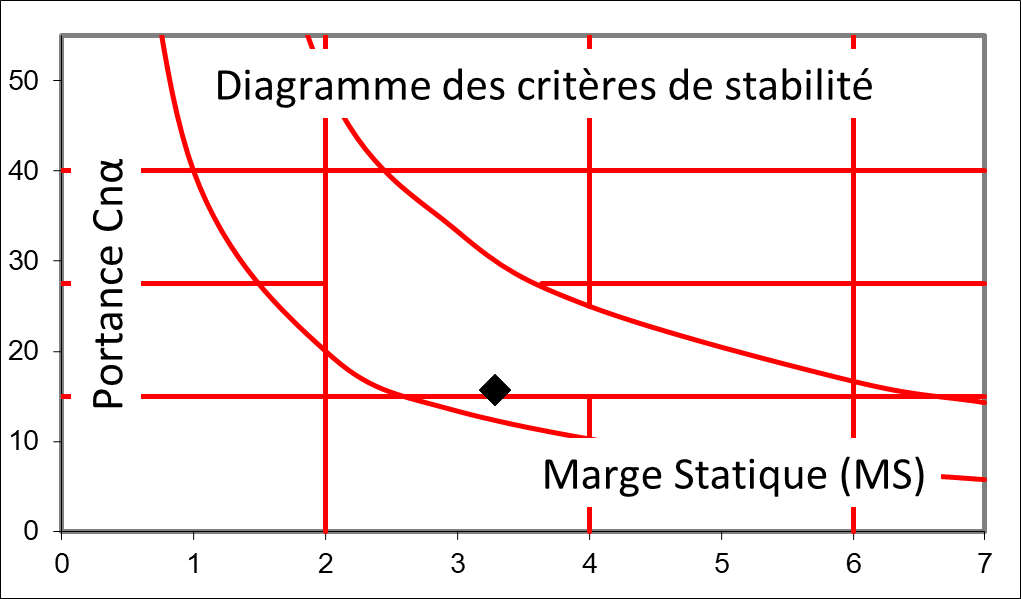
\includegraphics[width=\textwidth]{figures/stabtraj_alpha.png}
        \caption{Premier étage}
        \label{fig:stabilite_etage1}
    \end{subfigure}
    \begin{subfigure}{0.32\textwidth}
        \centering
        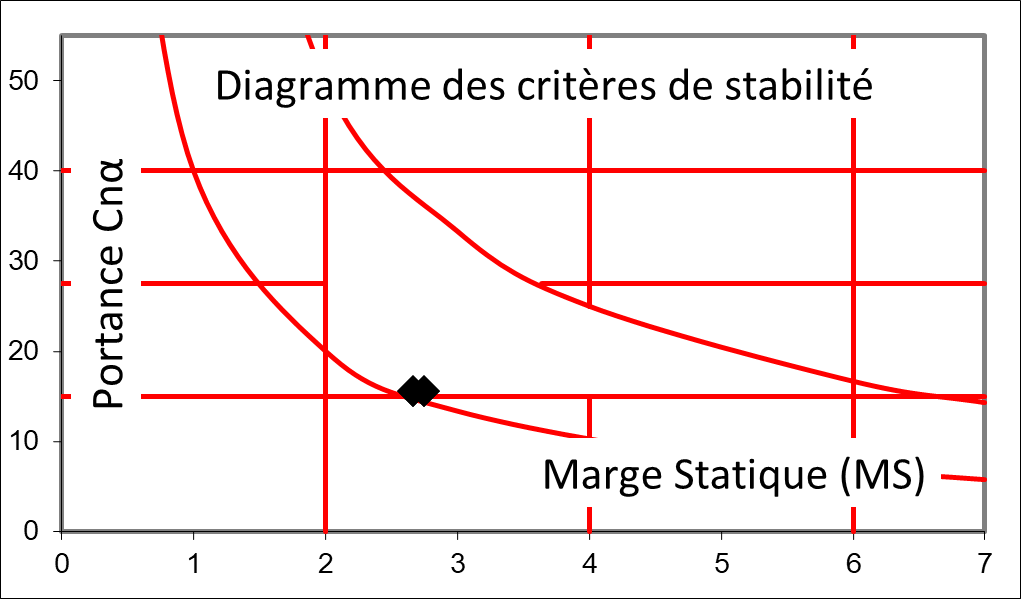
\includegraphics[width=\textwidth]{figures/stabtraj_beta.png}
        \caption{Second étage}
        \label{fig:stabilite_etage2}
    \end{subfigure}
    \caption{Résultats des analyses de stabilité longitudinale de la fusée SP-02 et de ses étages (\gls{Stabtraj})}
    \label{fig:stabilite_resultats}
\end{figure}

Nous observons que le graphique de la figure \ref{fig:stabilite_sp02} montre que les marges de stabilité de la fusée au complet
forment un prisme dû à l'effet de masquage. Ainsi, bien qu'une partie du prisme soit en dehors de la zone de stabilité (marge de
statique $< 2$), seule la droite supérieure du prisme à portance constante est celle effective. Cette droite étant incluse dans la
zone de stabilité, la fusée est donc stable durant toute sa phase de vol.\\

On remarque également que les marges de stabilité des deux étages individuellement, sont eux aussi stables bien que collés à la
limite inférieure de portance. Après discussion avec notre encadrant technique de la \acrshort{RCE}-1, il a été conclu que cette
situation était acceptable étant donné qu'au moment de la séparation des étages, ces deux étages auront déjà des vitesses
relativement élevées, assurant une stabilité dynamique suffisante malgré une portance faible.\\

Ces résultats ont été corrélés avec ceux obtenus via \gls{OpenRocket}, qui confirment la stabilité de la fusée.

\newpage
\subsubsubsection{Divergences de résultats avec les contrôles}
Pour confirmer notre étude de stabilité, nous devons confirmer nos résultats lors des contrôles au C'Space.
Nous verrons ici les divergences de valeurs et hypothèses avec le contrôle final et ainsi conclure l'étude.\\

\underline{Changements de dimensions}\\
Tout d'abord, vérifions les dimensions globales de la fusée complète et des deux étages entre les outils de conception (Stabtraj et OpenRocket) et le contrôle final.
Nous calculons dans chaque cas l'erreur relative entre l'outil utilisé et la réalité.\\
\begin{table}[h!]
    \centering
    \begin{tabular}{|l|l|l|l|l|}
        \hline
        \textbf{Fusée complète} & \textbf{Stabtraj} & \textbf{OpenRocket} & \textbf{Contrôle final} & \textbf{Erreur} \\
        \hline
        \textbf{Longueur (mm)} & 2252 & 2307 & 2290 & \textcolor{ForestGreen}{1,66 \%} | \textcolor{ForestGreen}{-0,74 \%}\\
        \hline
        \textbf{Centre de masse (mm)} & 1251 & 1295 & 1295 & \textcolor{YellowOrange}{3,39 \%} | \textcolor{ForestGreen}{\textbf{0,00 \%}}\\
        \hline
        \textbf{Masse (g)} & 7719 & 7719 & 7900 & \textcolor{ForestGreen}{2,29 \%} | \textcolor{ForestGreen}{2,29 \%} \\
        \hline
    \end{tabular}
    \caption{Résumé des gabarits de vol de la fusée SP-02 dans différentes configurations}
    \label{tab:gabarits_vol}
\end{table}

Pour la fusée complète, deux observations sont à noter :
\begin{itemize}
    \item L'erreur de longueur et du centre de masse sont liées à un allongement du second étage (+38mm) et corrigé dans l'estimation OpenRocket avec une masse identique,
    \item La longueur totale d'OpenRocket prend en compte la pointe en aluminium comme parfaite sans l'arrondi de l'entrée du capteur de pression.
\end{itemize}
\begin{table}[h!]
    \centering
    \begin{tabular}{|l|l|l|l|l|}
        \hline
        \textbf{1er étage} & \textbf{Stabtraj} & \textbf{OpenRocket} & \textbf{Contrôle final} & \textbf{Erreur} \\
        \hline
        \textbf{Longueur (mm)} & 1120 & 1125 & 1117 & \textcolor{ForestGreen}{-0,27 \%} | \textcolor{ForestGreen}{-0,72 \%}\\
        \hline
        \textbf{Centre de masse (mm)} & 542 & 493 & 520 & \textcolor{YellowOrange}{-4,23 \%} | \textcolor{Red}{5,19 \%}\\
        \hline
        \textbf{Masse (g)} & 4993 & 4341 & 4800 & \textcolor{YellowOrange}{-4,02 \%} | \textcolor{Red}{9,56 \%} \\
        \hline
    \end{tabular}
    \caption{Résumé des gabarits de vol de la fusée SP-02 dans différentes configurations}
    \label{tab:gabarits_vol}
\end{table}

Pour le premier étage, nous avons noté ici deux références de centre de masse avec une masse ajustée. Ce test nous a permis de calibrer l'étage entier.

\begin{table}[h!]
    \centering
    \begin{tabular}{|l|l|l|l|l|}
        \hline
        \textbf{2nd étage} & \textbf{Stabtraj} & \textbf{OpenRocket} & \textbf{Contrôle final} & \textbf{Erreur} \\
        \hline
        \textbf{Longueur (mm)} & 1177 & 1227 & 1217 & \textcolor{YellowOrange}{3,29 \%}   | \textcolor{ForestGreen}{-0,82 \%}\\
        \hline
        \textbf{Centre de masse (mm)} & 751 & 784 & 680 & \textcolor{Red}{-10,44 \%} | \textcolor{Red}{-15,29 \%}\\
        \hline
        \textbf{Masse (g)} & 3081 & 3228 & 3010 & \textcolor{ForestGreen}{-2,36 \%}  | \textcolor{Red}{-7,24 \%}\\
        \hline
    \end{tabular}
    \caption{Résumé des gabarits de vol de la fusée SP-02 dans différentes configurations}
    \label{tab:gabarits_vol}
\end{table}

Pour le second, nous avons dû changer le positionnement d'un bloc pour ainsi relever le centre de masse global et être cohérent avec la nouvelle longueur de l'étage. La masse globale n'a pas évoluée.\\

\underline{Changements d'hypothèses}\\
Également, nous noterons plusieurs changements dans les outils utilisés ainsi que dans les hypothèses d'étude définies :
\begin{itemize}
    \item Nous avons défini lors de l'étude notre diamètre de référence pondéré suivant la taille des étages, alors que dans le contrôle final c'est le plus petit diamètre qui a été choisi.\\ \underline{Conséquence :} Modification de l'emplacement du prisme de stabilité vers une surstabilité.
    \item Un changement de version du Stabtraj a modifié les données du Pro54 Barasinga, ainsi que le placement de la seconde paire d'ailerons (canards) qui est collée au tube dans la dernière version.\\ \underline{Conséquences :} Légères modifications des coefficients tels portance, marge statique, couple, $X_{Cp}$\ldots
\end{itemize}

\newpage